\chapter{The Rain of Blood}

As the jeweller returned to the apartment, he cast around him a
scrutinizing glance—but there was nothing to excite suspicion, if it
did not exist, or to confirm it, if it were already awakened.
Caderousse’s hands still grasped the gold and bank-notes, and La
Carconte called up her sweetest smiles while welcoming the reappearance
of their guest.

“‘Well, well,’ said the jeweller, ‘you seem, my good friends, to have
had some fears respecting the accuracy of your money, by counting it
over so carefully directly I was gone.’

“‘Oh, no,’ answered Caderousse, ‘that was not my reason, I can assure
you; but the circumstances by which we have become possessed of this
wealth are so unexpected, as to make us scarcely credit our good
fortune, and it is only by placing the actual proof of our riches
before our eyes that we can persuade ourselves that the whole affair is
not a dream.’

“The jeweller smiled. ‘Have you any other guests in your house?’
inquired he.

“‘Nobody but ourselves,’ replied Caderousse; ‘the fact is, we do not
lodge travellers—indeed, our tavern is so near the town, that nobody
would think of stopping here.’

“‘Then I am afraid I shall very much inconvenience you.’

“‘Inconvenience us? Not at all, my dear sir,’ said La Carconte in her
most gracious manner. ‘Not at all, I assure you.’

“‘But where will you manage to stow me?’

“‘In the chamber overhead.’

“‘Surely that is where you yourselves sleep?’

“‘Never mind that; we have a second bed in the adjoining room.’

“Caderousse stared at his wife with much astonishment.

“The jeweller, meanwhile, was humming a song as he stood warming his
back at the fire La Carconte had kindled to dry the wet garments of her
guest; and this done, she next occupied herself in arranging his
supper, by spreading a napkin at the end of the table, and placing on
it the slender remains of their dinner, to which she added three or
four fresh-laid eggs. Caderousse had once more parted with his
treasure—the banknotes were replaced in the pocket-book, the gold put
back into the bag, and the whole carefully locked in the cupboard. He
then began pacing the room with a pensive and gloomy air, glancing from
time to time at the jeweller, who stood reeking with the steam from his
wet clothes, and merely changing his place on the warm hearth, to
enable the whole of his garments to be dried.

“‘There,’ said La Carconte, as she placed a bottle of wine on the
table, ‘supper is ready whenever you are.’

“‘And you?’ asked Joannes.

“‘I don’t want any supper,’ said Caderousse.

“‘We dined so very late,’ hastily interposed La Carconte.

“‘Then it seems I am to eat alone,’ remarked the jeweller.

“‘Oh, we shall have the pleasure of waiting upon you,’ answered La
Carconte, with an eager attention she was not accustomed to manifest
even to guests who paid for what they took.

“From time to time Caderousse darted on his wife keen, searching
glances, but rapid as the lightning flash. The storm still continued.

“‘There, there,’ said La Carconte; ‘do you hear that? upon my word, you
did well to come back.’

“‘Nevertheless,’ replied the jeweller, ‘if by the time I have finished
my supper the tempest has at all abated, I shall make another start.’

“‘It’s the mistral,’ said Caderousse, ‘and it will be sure to last till
tomorrow morning.’ He sighed heavily.

“‘Well,’ said the jeweller, as he placed himself at table, ‘all I can
say is, so much the worse for those who are abroad.’

“‘Yes,’ chimed in La Carconte, ‘they will have a wretched night of it.’

“The jeweller began eating his supper, and the woman, who was
ordinarily so querulous and indifferent to all who approached her, was
suddenly transformed into the most smiling and attentive hostess. Had
the unhappy man on whom she lavished her assiduities been previously
acquainted with her, so sudden an alteration might well have excited
suspicion in his mind, or at least have greatly astonished him.
Caderousse, meanwhile, continued to pace the room in gloomy silence,
sedulously avoiding the sight of his guest; but as soon as the stranger
had completed his repast, the agitated innkeeper went eagerly to the
door and opened it.

“‘I believe the storm is over,’ said he.

“But as if to contradict his statement, at that instant a violent clap
of thunder seemed to shake the house to its very foundation, while a
sudden gust of wind, mingled with rain, extinguished the lamp he held
in his hand.

“Trembling and awe-struck, Caderousse hastily shut the door and
returned to his guest, while La Carconte lighted a candle by the
smouldering ashes that glimmered on the hearth.

“‘You must be tired,’ said she to the jeweller; ‘I have spread a pair
of white sheets on your bed; go up when you are ready, and sleep well.’

“Joannes stayed for a while to see whether the storm seemed to abate in
its fury, but a brief space of time sufficed to assure him that,
instead of diminishing, the violence of the rain and thunder
momentarily increased; resigning himself, therefore, to what seemed
inevitable, he bade his host good-night, and mounted the stairs. He
passed over my head and I heard the flooring creak beneath his
footsteps. The quick, eager glance of La Carconte followed him as he
ascended, while Caderousse, on the contrary, turned his back, and
seemed most anxiously to avoid even glancing at him.

“All these circumstances did not strike me as painfully at the time as
they have since done; in fact, all that had happened (with the
exception of the story of the diamond, which certainly did wear an air
of improbability), appeared natural enough, and called for neither
apprehension nor mistrust; but, worn out as I was with fatigue, and
fully purposing to proceed onwards directly the tempest abated, I
determined to obtain a few hours’ sleep. Overhead I could accurately
distinguish every movement of the jeweller, who, after making the best
arrangements in his power for passing a comfortable night, threw
himself on his bed, and I could hear it creak and groan beneath his
weight.

“Insensibly my eyelids grew heavy, deep sleep stole over me, and having
no suspicion of anything wrong, I sought not to shake it off. I looked
into the kitchen once more and saw Caderousse sitting by the side of a
long table upon one of the low wooden stools which in country places
are frequently used instead of chairs; his back was turned towards me,
so that I could not see the expression of his countenance—neither
should I have been able to do so had he been placed differently, as his
head was buried between his two hands. La Carconte continued to gaze on
him for some time, then shrugging her shoulders, she took her seat
immediately opposite to him.

“At this moment the expiring embers threw up a fresh flame from the
kindling of a piece of wood that lay near, and a bright light flashed
over the room. La Carconte still kept her eyes fixed on her husband,
but as he made no sign of changing his position, she extended her hard,
bony hand, and touched him on the forehead.

\begin{figure}[ht]
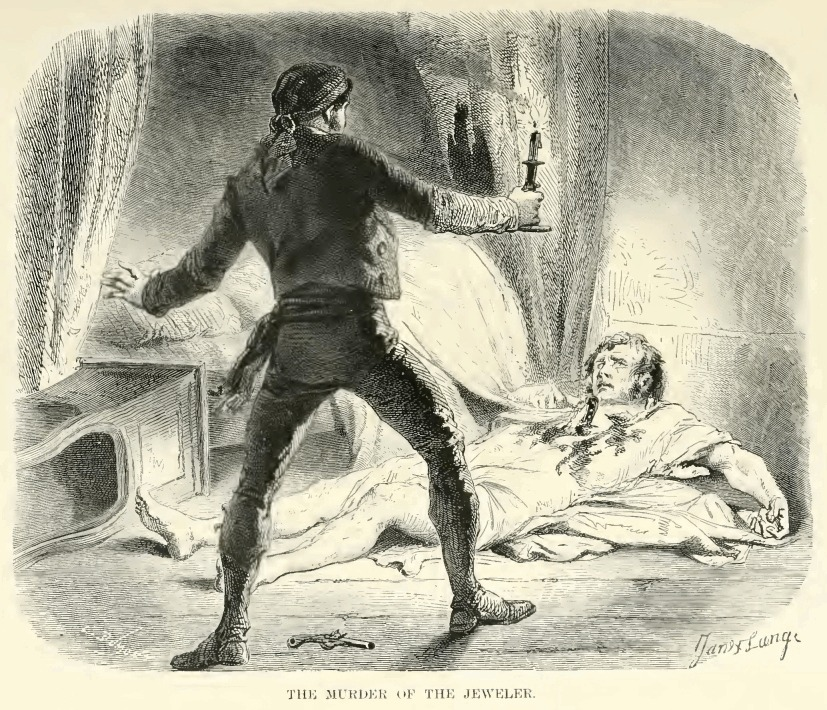
\includegraphics[width=\textwidth]{20317m.jpg}
\end{figure}

“Caderousse shuddered. The woman’s lips seemed to move, as though she
were talking; but because she merely spoke in an undertone, or my
senses were dulled by sleep, I did not catch a word she uttered.
Confused sights and sounds seemed to float before me, and gradually I
fell into a deep, heavy slumber. How long I had been in this
unconscious state I know not, when I was suddenly aroused by the report
of a pistol, followed by a fearful cry. Weak and tottering footsteps
resounded across the chamber above me, and the next instant a dull,
heavy weight seemed to fall powerless on the staircase. I had not yet
fully recovered consciousness, when again I heard groans, mingled with
half-stifled cries, as if from persons engaged in a deadly struggle. A
cry more prolonged than the others and ending in a series of groans
effectually roused me from my drowsy lethargy. Hastily raising myself
on one arm, I looked around, but all was dark; and it seemed to me as
if the rain must have penetrated through the flooring of the room
above, for some kind of moisture appeared to fall, drop by drop, upon
my forehead, and when I passed my hand across my brow, I felt that it
was wet and clammy.

“To the fearful noises that had awakened me had succeeded the most
perfect silence—unbroken, save by the footsteps of a man walking about
in the chamber above. The staircase creaked, he descended into the room
below, approached the fire and lit a candle.

“The man was Caderousse—he was pale and his shirt was all bloody.
Having obtained the light, he hurried upstairs again, and once more I
heard his rapid and uneasy footsteps.

“A moment later he came down again, holding in his hand the small
shagreen case, which he opened, to assure himself it contained the
diamond,—seemed to hesitate as to which pocket he should put it in,
then, as if dissatisfied with the security of either pocket, he
deposited it in his red handkerchief, which he carefully rolled round
his head.

“After this he took from his cupboard the bank-notes and gold he had
put there, thrust the one into the pocket of his trousers, and the
other into that of his waistcoat, hastily tied up a small bundle of
linen, and rushing towards the door, disappeared in the darkness of the
night.

“Then all became clear and manifest to me, and I reproached myself with
what had happened, as though I myself had done the guilty deed. I
fancied that I still heard faint moans, and imagining that the
unfortunate jeweller might not be quite dead, I determined to go to his
relief, by way of atoning in some slight degree, not for the crime I
had committed, but for that which I had not endeavored to prevent. For
this purpose I applied all the strength I possessed to force an
entrance from the cramped spot in which I lay to the adjoining room.
The poorly fastened boards which alone divided me from it yielded to my
efforts, and I found myself in the house. Hastily snatching up the
lighted candle, I hurried to the staircase; about midway a body was
lying quite across the stairs. It was that of La Carconte. The pistol I
had heard had doubtless been fired at her. The shot had frightfully
lacerated her throat, leaving two gaping wounds from which, as well as
the mouth, the blood was pouring in floods. She was stone dead. I
strode past her, and ascended to the sleeping chamber, which presented
an appearance of the wildest disorder. The furniture had been knocked
over in the deadly struggle that had taken place there, and the sheets,
to which the unfortunate jeweller had doubtless clung, were dragged
across the room. The murdered man lay on the floor, his head leaning
against the wall, and about him was a pool of blood which poured forth
from three large wounds in his breast; there was a fourth gash, in
which a long table knife was plunged up to the handle.

“I stumbled over some object; I stooped to examine—it was the second
pistol, which had not gone off, probably from the powder being wet. I
approached the jeweller, who was not quite dead, and at the sound of my
footsteps and the creaking of the floor, he opened his eyes, fixed them
on me with an anxious and inquiring gaze, moved his lips as though
trying to speak, then, overcome by the effort, fell back and expired.

“This appalling sight almost bereft me of my senses, and finding that I
could no longer be of service to anyone in the house, my only desire
was to fly. I rushed towards the staircase, clutching my hair, and
uttering a groan of horror.

“Upon reaching the room below, I found five or six custom-house
officers, and two or three gendarmes—all heavily armed. They threw
themselves upon me. I made no resistance; I was no longer master of my
senses. When I strove to speak, a few inarticulate sounds alone escaped
my lips.

“As I noticed the significant manner in which the whole party pointed
to my blood-stained garments, I involuntarily surveyed myself, and then
I discovered that the thick warm drops that had so bedewed me as I lay
beneath the staircase must have been the blood of La Carconte. I
pointed to the spot where I had concealed myself.

“‘What does he mean?’ asked a gendarme.

“One of the officers went to the place I directed.

“‘He means,’ replied the man upon his return, ‘that he got in that
way;’ and he showed the hole I had made when I broke through.

“Then I saw that they took me for the assassin. I recovered force and
energy enough to free myself from the hands of those who held me, while
I managed to stammer forth:

“‘I did not do it! Indeed, indeed I did not!’

“A couple of gendarmes held the muzzles of their carbines against my
breast.

“‘Stir but a step,’ said they, ‘and you are a dead man.’

“‘Why should you threaten me with death,’ cried I, ‘when I have already
declared my innocence?’

“‘Tush, tush,’ cried the men; ‘keep your innocent stories to tell to
the judge at Nîmes. Meanwhile, come along with us; and the best advice
we can give you is to do so unresistingly.’

“Alas, resistance was far from my thoughts. I was utterly overpowered
by surprise and terror; and without a word I suffered myself to be
handcuffed and tied to a horse’s tail, and thus they took me to Nîmes.

“I had been tracked by a customs-officer, who had lost sight of me near
the tavern; feeling certain that I intended to pass the night there, he
had returned to summon his comrades, who just arrived in time to hear
the report of the pistol, and to take me in the midst of such
circumstantial proofs of my guilt as rendered all hopes of proving my
innocence utterly futile. One only chance was left me, that of
beseeching the magistrate before whom I was taken to cause every
inquiry to be made for the Abbé Busoni, who had stopped at the inn of
the Pont du Gard on that morning.

“If Caderousse had invented the story relative to the diamond, and
there existed no such person as the Abbé Busoni, then, indeed, I was
lost past redemption, or, at least, my life hung upon the feeble chance
of Caderousse himself being apprehended and confessing the whole truth.

“Two months passed away in hopeless expectation on my part, while I
must do the magistrate the justice to say that he used every means to
obtain information of the person I declared could exculpate me if he
would. Caderousse still evaded all pursuit, and I had resigned myself
to what seemed my inevitable fate. My trial was to come on at the
approaching assizes; when, on the 8th of September—that is to say,
precisely three months and five days after the events which had
perilled my life—the Abbé Busoni, whom I never ventured to believe I
should see, presented himself at the prison doors, saying he understood
one of the prisoners wished to speak to him; he added, that having
learned at Marseilles the particulars of my imprisonment, he hastened
to comply with my desire.

“You may easily imagine with what eagerness I welcomed him, and how
minutely I related the whole of what I had seen and heard. I felt some
degree of nervousness as I entered upon the history of the diamond,
but, to my inexpressible astonishment, he confirmed it in every
particular, and to my equal surprise, he seemed to place entire belief
in all I said.

“And then it was that, won by his mild charity, seeing that he was
acquainted with all the habits and customs of my own country, and
considering also that pardon for the only crime of which I was really
guilty might come with a double power from lips so benevolent and kind,
I besought him to receive my confession, under the seal of which I
recounted the Auteuil affair in all its details, as well as every other
transaction of my life. That which I had done by the impulse of my best
feelings produced the same effect as though it had been the result of
calculation. My voluntary confession of the assassination at Auteuil
proved to him that I had not committed that of which I stood accused.
When he quitted me, he bade me be of good courage, and to rely upon his
doing all in his power to convince my judges of my innocence.

“I had speedy proofs that the excellent abbé was engaged in my behalf,
for the rigors of my imprisonment were alleviated by many trifling
though acceptable indulgences, and I was told that my trial was to be
postponed to the assizes following those now being held.

“In the interim it pleased Providence to cause the apprehension of
Caderousse, who was discovered in some distant country, and brought
back to France, where he made a full confession, refusing to make the
fact of his wife’s having suggested and arranged the murder any excuse
for his own guilt. The wretched man was sentenced to the galleys for
life, and I was immediately set at liberty.”

“And then it was, I presume,” said Monte Cristo “that you came to me as
the bearer of a letter from the Abbé Busoni?”

“It was, your excellency; the benevolent abbé took an evident interest
in all that concerned me.

“‘Your mode of life as a smuggler,’ said he to me one day, ‘will be the
ruin of you; if you get out, don’t take it up again.’

“‘But how,’ inquired I, ‘am I to maintain myself and my poor sister?’

“‘A person, whose confessor I am,’ replied he, ‘and who entertains a
high regard for me, applied to me a short time since to procure him a
confidential servant. Would you like such a post? If so, I will give
you a letter of introduction to him.’

“‘Oh, father,’ I exclaimed, ‘you are very good.’

“‘But you must swear solemnly that I shall never have reason to repent
my recommendation.’

“I extended my hand, and was about to pledge myself by any promise he
would dictate, but he stopped me.

“‘It is unnecessary for you to bind yourself by any vow,’ said he; ‘I
know and admire the Corsican nature too well to fear you. Here, take
this,’ continued he, after rapidly writing the few lines I brought to
your excellency, and upon receipt of which you deigned to receive me
into your service, and proudly I ask whether your excellency has ever
had cause to repent having done so?”

“No,” replied the count; “I take pleasure in saying that you have
served me faithfully, Bertuccio; but you might have shown more
confidence in me.”

“I, your excellency?”

“Yes; you. How comes it, that having both a sister and an adopted son,
you have never spoken to me of either?”

\begin{figure}[ht]
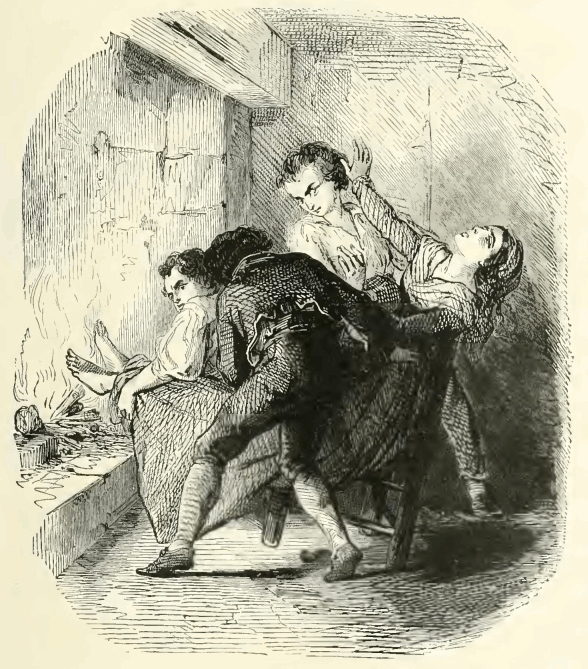
\includegraphics[width=\textwidth]{20323m.jpg}
\end{figure}

“Alas, I have still to recount the most distressing period of my life.
Anxious as you may suppose I was to behold and comfort my dear sister,
I lost no time in hastening to Corsica, but when I arrived at Rogliano
I found a house of mourning, the consequences of a scene so horrible
that the neighbors remember and speak of it to this day. Acting by my
advice, my poor sister had refused to comply with the unreasonable
demands of Benedetto, who was continually tormenting her for money, as
long as he believed there was a sou left in her possession. One morning
he threatened her with the severest consequences if she did not supply
him with what he desired, and disappeared and remained away all day,
leaving the kind-hearted Assunta, who loved him as if he were her own
child, to weep over his conduct and bewail his absence. Evening came,
and still, with all the patient solicitude of a mother, she watched for
his return.

“As the eleventh hour struck, he entered with a swaggering air,
attended by two of the most dissolute and reckless of his boon
companions. She stretched out her arms to him, but they seized hold of
her, and one of the three—none other than the accursed Benedetto
exclaimed:

“‘Put her to torture and she’ll soon tell us where her money is.’

“It unfortunately happened that our neighbor, Wasilio, was at Bastia,
leaving no person in his house but his wife; no human creature beside
could hear or see anything that took place within our dwelling. Two
held poor Assunta, who, unable to conceive that any harm was intended
to her, smiled in the face of those who were soon to become her
executioners. The third proceeded to barricade the doors and windows,
then returned, and the three united in stifling the cries of terror
incited by the sight of these preparations, and then dragged Assunta
feet foremost towards the brazier, expecting to wring from her an
avowal of where her supposed treasure was secreted. In the struggle her
clothes caught fire, and they were obliged to let go their hold in
order to preserve themselves from sharing the same fate. Covered with
flames, Assunta rushed wildly to the door, but it was fastened; she
flew to the windows, but they were also secured; then the neighbors
heard frightful shrieks; it was Assunta calling for help. The cries
died away in groans, and next morning, as soon as Wasilio’s wife could
muster up courage to venture abroad, she caused the door of our
dwelling to be opened by the public authorities, when Assunta, although
dreadfully burnt, was found still breathing; every drawer and closet in
the house had been forced open, and the money stolen. Benedetto never
again appeared at Rogliano, neither have I since that day either seen
or heard anything concerning him.

“It was subsequently to these dreadful events that I waited on your
excellency, to whom it would have been folly to have mentioned
Benedetto, since all trace of him seemed entirely lost; or of my
sister, since she was dead.”

“And in what light did you view the occurrence?” inquired Monte Cristo.

“As a punishment for the crime I had committed,” answered Bertuccio.
“Oh, those Villeforts are an accursed race!”

“Truly they are,” murmured the count in a lugubrious tone.

“And now,” resumed Bertuccio, “your excellency may, perhaps, be able to
comprehend that this place, which I revisit for the first time—this
garden, the actual scene of my crime—must have given rise to
reflections of no very agreeable nature, and produced that gloom and
depression of spirits which excited the notice of your excellency, who
was pleased to express a desire to know the cause. At this instant a
shudder passes over me as I reflect that possibly I am now standing on
the very grave in which lies M. de Villefort, by whose hand the ground
was dug to receive the corpse of his child.”

“Everything is possible,” said Monte Cristo, rising from the bench on
which he had been sitting; “even,” he added in an inaudible voice,
“even that the procureur be not dead. The Abbé Busoni did right to send
you to me,” he went on in his ordinary tone, “and you have done well in
relating to me the whole of your history, as it will prevent my forming
any erroneous opinions concerning you in future. As for that Benedetto,
who so grossly belied his name, have you never made any effort to trace
out whither he has gone, or what has become of him?”

“No; far from wishing to learn whither he has betaken himself, I should
shun the possibility of meeting him as I would a wild beast. Thank God,
I have never heard his name mentioned by any person, and I hope and
believe he is dead.”

“Do not think so, Bertuccio,” replied the count; “for the wicked are
not so easily disposed of, for God seems to have them under his special
watch-care to make of them instruments of his vengeance.”

“So be it,” responded Bertuccio, “all I ask of heaven is that I may
never see him again. And now, your excellency,” he added, bowing his
head, “you know everything—you are my judge on earth, as the Almighty
is in heaven; have you for me no words of consolation?”

“My good friend, I can only repeat the words addressed to you by the
Abbé Busoni. Villefort merited punishment for what he had done to you,
and, perhaps, to others. Benedetto, if still living, will become the
instrument of divine retribution in some way or other, and then be duly
punished in his turn. As far as you yourself are concerned, I see but
one point in which you are really guilty. Ask yourself, wherefore,
after rescuing the infant from its living grave, you did not restore it
to its mother? There was the crime, Bertuccio—that was where you became
really culpable.”

“True, excellency, that was the crime, the real crime, for in that I
acted like a coward. My first duty, directly I had succeeded in
recalling the babe to life, was to restore it to its mother; but, in
order to do so, I must have made close and careful inquiry, which
would, in all probability, have led to my own apprehension; and I clung
to life, partly on my sister’s account, and partly from that feeling of
pride inborn in our hearts of desiring to come off untouched and
victorious in the execution of our vengeance. Perhaps, too, the natural
and instinctive love of life made me wish to avoid endangering my own.
And then, again, I am not as brave and courageous as was my poor
brother.”

Bertuccio hid his face in his hands as he uttered these words, while
Monte Cristo fixed on him a look of inscrutable meaning. After a brief
silence, rendered still more solemn by the time and place, the count
said, in a tone of melancholy wholly unlike his usual manner:

“In order to bring this conversation to a fitting termination (the last
we shall ever hold upon this subject), I will repeat to you some words
I have heard from the lips of the Abbé Busoni. For all evils there are
two remedies—time and silence. And now leave me, Monsieur Bertuccio, to
walk alone here in the garden. The very circumstances which inflict on
you, as a principal in the tragic scene enacted here, such painful
emotions, are to me, on the contrary, a source of something like
contentment, and serve but to enhance the value of this dwelling in my
estimation. The chief beauty of trees consists in the deep shadow of
their umbrageous boughs, while fancy pictures a moving multitude of
shapes and forms flitting and passing beneath that shade. Here I have a
garden laid out in such a way as to afford the fullest scope for the
imagination, and furnished with thickly grown trees, beneath whose
leafy screen a visionary like myself may conjure up phantoms at will.
This to me, who expected but to find a blank enclosure surrounded by a
straight wall, is, I assure you, a most agreeable surprise. I have no
fear of ghosts, and I have never heard it said that so much harm had
been done by the dead during six thousand years as is wrought by the
living in a single day. Retire within, Bertuccio, and tranquillize your
mind. Should your confessor be less indulgent to you in your dying
moments than you found the Abbé Busoni, send for me, if I am still on
earth, and I will soothe your ears with words that shall effectually
calm and soothe your parting soul ere it goes forth to traverse the
ocean called eternity.”

Bertuccio bowed respectfully, and turned away, sighing heavily. Monte
Cristo, left alone, took three or four steps onwards, and murmured:

“Here, beneath this plane-tree, must have been where the infant’s grave
was dug. There is the little door opening into the garden. At this
corner is the private staircase communicating with the sleeping
apartment. There will be no necessity for me to make a note of these
particulars, for there, before my eyes, beneath my feet, all around me,
I have the plan sketched with all the living reality of truth.”

After making the tour of the garden a second time, the count re-entered
his carriage, while Bertuccio, who perceived the thoughtful expression
of his master’s features, took his seat beside the driver without
uttering a word. The carriage proceeded rapidly towards Paris.

That same evening, upon reaching his abode in the Champs-Élysées, the
Count of Monte Cristo went over the whole building with the air of one
long acquainted with each nook or corner. Nor, although preceding the
party, did he once mistake one door for another, or commit the smallest
error when choosing any particular corridor or staircase to conduct him
to a place or suite of rooms he desired to visit. Ali was his principal
attendant during this nocturnal survey. Having given various orders to
Bertuccio relative to the improvements and alterations he desired to
make in the house, the Count, drawing out his watch, said to the
attentive Nubian:

“It is half-past eleven o’clock; Haydée will soon be here. Have the
French attendants been summoned to await her coming?”

Ali extended his hands towards the apartments destined for the fair
Greek, which were so effectually concealed by means of a tapestried
entrance, that it would have puzzled the most curious to have divined
their existence. Ali, having pointed to the apartments, held up three
fingers of his right hand, and then, placing it beneath his head, shut
his eyes, and feigned to sleep.

“I understand,” said Monte Cristo, well acquainted with Ali’s
pantomime; “you mean to tell me that three female attendants await
their new mistress in her sleeping-chamber.”

Ali, with considerable animation, made a sign in the affirmative.

“Madame will be tired tonight,” continued Monte Cristo, “and will, no
doubt, wish to rest. Desire the French attendants not to weary her with
questions, but merely to pay their respectful duty and retire. You will
also see that the Greek servants hold no communication with those of
this country.”

He bowed. Just at that moment voices were heard hailing the concierge.
The gate opened, a carriage rolled down the avenue, and stopped at the
steps. The count hastily descended, presented himself at the already
opened carriage door, and held out his hand to a young woman,
completely enveloped in a green silk mantle heavily embroidered with
gold. She raised the hand extended towards her to her lips, and kissed
it with a mixture of love and respect. Some few words passed between
them in that sonorous language in which Homer makes his gods converse.
The young woman spoke with an expression of deep tenderness, while the
count replied with an air of gentle gravity.

Preceded by Ali, who carried a rose-colored flambeau in his hand, the
young lady, who was no other than the lovely Greek who had been Monte
Cristo’s companion in Italy, was conducted to her apartments, while the
count retired to the pavilion reserved for himself. In another hour
every light in the house was extinguished, and it might have been
thought that all its inmates slept.
